\section{Enterprise Resource Planning}

ERP systems often feature vertical solutions specifically designed to meet the needs of different industries. 
These solutions are tailored to be highly specialized.
However, we can make a broader distinction between manufacturing and service companies:
\begin{itemize}
    \item Manufacturing companies produce tangible products.
    \item Service companies provide intangible products.
\end{itemize}

\subsection{Manufactoring companies}
Manufacturing companies typically rely on three main functional portfolios within their ERP systems:
\begin{enumerate}
    \item Administrative portfolio.
    \item Operational portfolio.
    \item Executive portfolio.
\end{enumerate}
\noindent These portfolios, while initially developed separately, are now integrated within modern ERP systems, forming the core functionalities of these systems.

\begin{figure}[H]
    \centering
    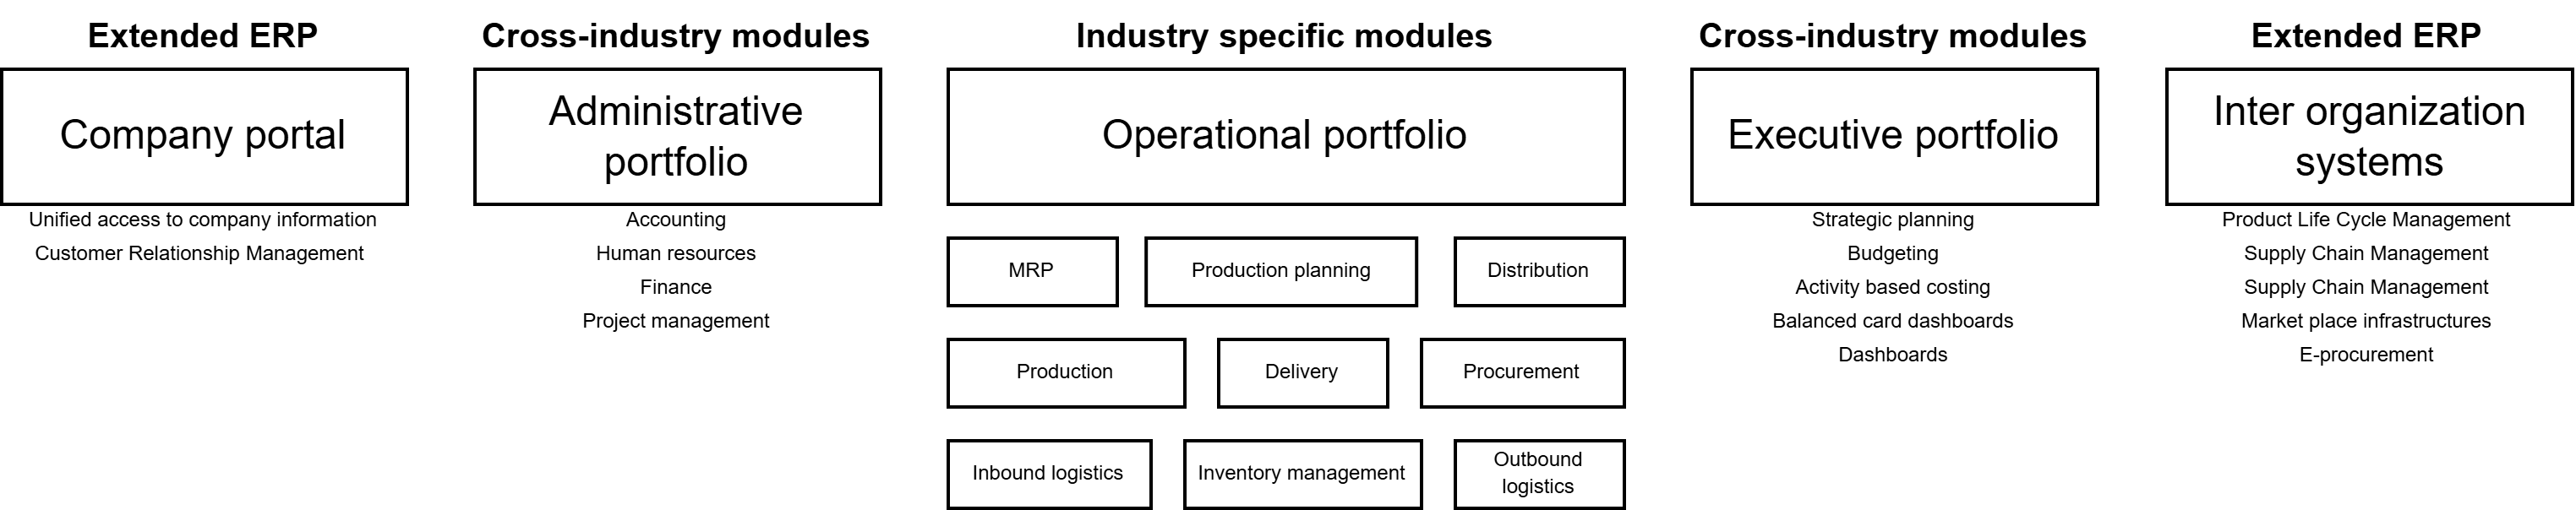
\includegraphics[width=0.5\linewidth]{images/bis1.png}
    \caption{ERP functional architecture}
\end{figure}

\subsection{Administrative portfolio}
The administrative portfolio focuses on automating organizational activities that are often administrative and bureaucratic in nature, including: accounting and tax management, finance, human resources, project management (from an accounting perspective), and governmental procedures.

This portfolio is largely industry-agnostic, although it is country-specific. 
It represents an early stage of automation, alongside office automation, by streamlining tasks that involve number crunching. 
It typically involves minimal decision-making, as its processes are procedural and repetitive. 
Although traditionally viewed as stand-alone, it often links to other processes, such as activity-based costing.

Despite its simplicity in design, the administrative portfolio can be functionally complex.